\documentclass[11pt,a4paper,twoside]{article}
\usepackage[margin=1in, headheight=14pt]{geometry}
\usepackage{amsfonts,amsmath,amssymb,suetterl}
\usepackage{lmodern}
\usepackage[T1]{fontenc}
\usepackage{fancyhdr}
\usepackage{float}
\usepackage[utf8]{inputenc}
\usepackage{fontawesome}
\usepackage{enumerate}
\usepackage{physics}
\usepackage{tikz}

\DeclareUnicodeCharacter{2212}{-}

\usepackage{mathrsfs}
\usepackage[nodisplayskipstretch]{setspace}

\setstretch{1.5}
\renewcommand{\footrulewidth}{0pt}

\parindent 0ex
\setlength{\parskip}{1em}

\fancyfoot{}
\raggedbottom

\begin{document}
    %
	\begin{singlespace}
		\begin{center}
			\Huge Queen Mary\\
			\LARGE University of London
		\end{center}
		\Large \textbf{MTH5123} \hfill \Large \textbf{Differential Equations,} \hfill \Large \textbf{Fall 2020}\\
		\large \textbf{Coursework 4: part 2 week 9 - Selected Solutions} \hfill \large \textbf{W. Huang}
		%
		\rule{\textwidth}{0.4pt}
	\end{singlespace}
	\textbf{I. Tutorial Problems}\par
	%
	\begin{enumerate}[\bfseries A.]
		\item Determine the eigenvalues and eigenvectors of the following matrices:
		$$
		\begin{bmatrix}
			0 & -1\\
			-1 & 0
		\end{bmatrix}\quad
		\begin{bmatrix}
			2 & 0\\
			0 & -3
		\end{bmatrix}\quad
		\begin{bmatrix}
			1 & 1\\
			4 & 1
		\end{bmatrix}
		$$
		\textbf{Solution:} In each case, we first find the eigenvalues $\lambda$ using $\det(A = \lambda I_{2\times 2}) = 0$ and then for each $\lambda$, determine an associated eigenvector $\vec{v}$ satisfying $A\vec{v} = \lambda \vec{v}$.
		\begin{align*}
			\begin{bmatrix}
				0 & 1\\
				-1 & 0
			\end{bmatrix}\quad
			&\Rightarrow \quad
			\lambda = \pm i,\quad v_1 =
			\begin{bmatrix}
				-i\\
				1
			\end{bmatrix},\ v_2 = 
			\begin{bmatrix}
				i\\1
			\end{bmatrix}\\
			\begin{bmatrix}
				2 & 0\\
				0 & -3
			\end{bmatrix}\quad
			&\Rightarrow \quad
			\lambda = 2,\ -3,\quad v_1 =
			\begin{bmatrix}
				1\\
				0
			\end{bmatrix},\ v_2=
			\begin{bmatrix}
				0\\
				1
			\end{bmatrix}\\
			\begin{bmatrix}
				1 & 1\\
				1 & 4
			\end{bmatrix}\quad
			&\Rightarrow \quad
			\lambda = 3,\ -1,\quad v_1 =
			\begin{bmatrix}
				1\\
				2
			\end{bmatrix},\ v_2 =
			\begin{bmatrix}
				-1\\
				2
			\end{bmatrix}.
		\end{align*}
		\item Find and sketch the solution of the following initial value problems
		\begin{enumerate}[\bfseries 1)]
			\item $\dot{y_1} = -\frac{1}{2}y_1 + \frac{5}{2}y_2,\ \dot{y_2} = \frac{5}{2}y_1 - \frac{1}{2}y_2,\ y_1(0) = a,\ y_2(0) = b$.\par
			\textbf{Solution.} The matrix associated with this system is given by
			$
			A = 
			\begin{bmatrix}
				-\frac{1}{2} & \frac{5}{2}\\
				\frac{5}{2} & -\frac{1}{2}
			\end{bmatrix}.
			$
			The characteristic equation is $\lambda^2 + \lambda - 6 = 0$ with two positive real roots $\lambda_1 = 2,\ \lambda_2 = -3$. The eigenvector corresponding to $\lambda_1 = 2$ can be found from
			$$
			\begin{pmatrix}
				-\frac{1}{2} & \frac{5}{2}\\
				\frac{5}{2} & -\frac{1}{2}
			\end{pmatrix}
			\begin{pmatrix}
				p_1 \\
				q_1
			\end{pmatrix} -2
			\begin{pmatrix}
				p_1\\
				q_1
			\end{pmatrix}\quad q_1 = p_1\quad
			$$
			so that
			$
			\vb{u_1} =
			\begin{pmatrix}
				1\\
				1
			\end{pmatrix}
			$.
			Similarly, for $\lambda_1 = −3$ we find $q_2 = -p_2$ so that the eigenvector is
			$
			\vb{u_2} =
			\begin{pmatrix}
				1\\
				-1
			\end{pmatrix}
			$.
			The general solution has the form
			$$
			\begin{pmatrix}
				y_1\\
				y_2
			\end{pmatrix}
			=
			C_1e^{2t}
			\begin{pmatrix}
				1\\
				1
			\end{pmatrix} + C_2e^{-3t}
			\begin{pmatrix}
				1\\
				-1
			\end{pmatrix}.
			$$
			The initial conditions yield
			$$
			y_1(0) = C_1 + C_2 = a,\ y_2(0) = C_1 - C_2=b \Rightarrow C_1 = \frac{1}{2}(a+b),\ C_2 = \frac{1}{2}(a-b)
			$$
			so that the solution to the initial value problem is given by
			$$
			y_1 = \frac{1}{2}(a+b)e^{2t} + \frac{1}{2}(a-b)e^{-3t},\ y_2 = \frac{1}{2}(a+b)e^{2t}-\frac{1}{2}(a-b)e^{-3t}.
			$$
			Sketch the solution to the IVP when $y_1(0) = a,\ y_2(0) = b$. (This is what we practiced in CW7, where we plotted the parametric curves based on $y_1(t)$ and $y_2(t)$.) By varying the values of $(a, b)$ in the initial conditions, we have the solutions are sketched as follow,
			\begin{figure}[!h]
				\centering
					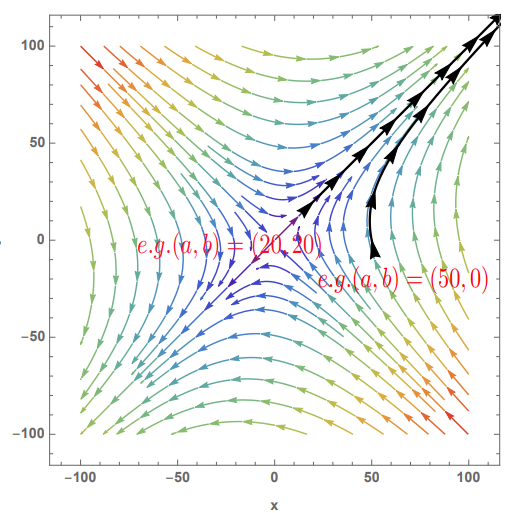
\includegraphics[width=0.50\textwidth]{figure/pdf24B1.PNG}
			\end{figure}
			where we marked two example trajectories (solutions) to two different initial conditions as $y_1(0) = a = 20,\ y_2(0) = b = 20$, and $y_1(0) = a = 50,\ y_2(0) = b = 0$.\\
			(Note: In our lecture, we explained when the initial conditions are not fixed numbers yet, we can plot solutions by assuming different values of $a$ and $b$. This will refer to different initial conditions thus different solutions in the phase plane. Once you tried enough initial conditions, you will get a rough picture of the all possible solutions, which become the phase portrait (general solution) to the ODE system. Connect this practice with our week 10 lectures.)
			%
			\item $\dot{y_1} = -y_1 + 5y_2,\ \dot{y_2} = -y_1 + y_2,\ y_1(0) = 0,\ y_2(0) = 4$.\par
			\textbf{Solution.} The matrix associated with this system is given by
			$
			A =
			\begin{pmatrix}
				-1 & 5\\
				-1 & 1
			\end{pmatrix}
			$.
			The characteristic equation is $\lambda_2 + 4 = 0$ with two complex conjugate roots $\lambda_1 = 2i,\ \lambda_2 = −2i$. The eigenvector corresponding to $\lambda_1 = 2i$ can be found from
			$$
			\begin{pmatrix}
				-1 & 5\\
				-1 & 1
			\end{pmatrix}
			\begin{pmatrix}
				p_1\\
				q_1
			\end{pmatrix}
			= 2i
			\begin{pmatrix}
				p_1\\
				q_1
			\end{pmatrix}\ \Rightarrow\ 
			5q_1 = (1+2i)p_1
			$$
			so that the eigenvectors are
			$
			\vb{u_1} =
			\begin{pmatrix}
				1\\
				\frac{1}{5}(1+2i)
			\end{pmatrix}
			$
			and the complex conjugate vector
			$
			\vb{u_2} =
			\begin{pmatrix}
				1\\
				\frac{1}{5}(1-2i)
			\end{pmatrix}
			$.
			The general solution has the form
			$$
			\begin{pmatrix}
				y_1\\
				y
			\end{pmatrix}
			= C_1e^{2it}
			\begin{pmatrix}
				1\\
				\frac{1}{5}(1+2i)
			\end{pmatrix} + C_2e^{-2it}
			\begin{pmatrix}
				1\\
				\frac{1}{5}(1-2i)
			\end{pmatrix}.
			$$
			The initial conditions yield
			$$
			y_1(0) = C1 + C2 = 0,\ y_2(0) = C_1\frac{1}{5}(1+ 2i) + C_2\frac{1}{5}(1-2i) =4,\ \Rightarrow C_1 = -5i,\ C_2 = 5i.
			$$
			The solution $y_1(t)$ to the initial value problem is given by
			$$
			y_1 = -5u(e^{2it} - e^{-2it}) = 10\sin 2t.
			$$
			Similarly we have
			$$
			y_2 = -\frac{5i}{5}(1+2i)e^{2it} + \frac{5i}{5}(1-2i)e^{-2it} = -i(e^{2it} + 2i(e^{2it} + e^{-2it}))
			$$
			so that
			$$
			y_2 = 2\sin 2t + 4\cos 2t.
			$$
			\begin{figure}[!h]
				\centering
					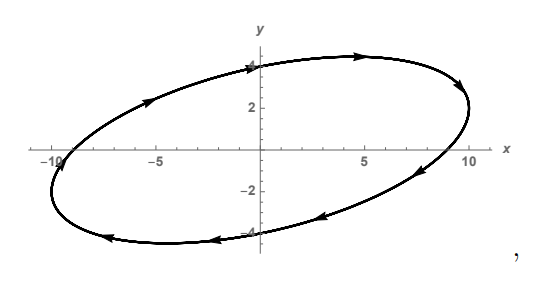
\includegraphics[width=0.50\textwidth]{figure/pdf24B2.PNG}
			\end{figure}
		\end{enumerate}
		\item
		\begin{enumerate}[\bfseries (1)]
			\item Linearize $\dot{y_1} = y_1+e^y_2-\cos y_2,\ \dot{y_2} = 3y_1 - y_2-\sin y_2$ around the fixed point at $y_1 = y_2 = 0$.\par
			\textbf{Solution.} We first linearize this system around $y_1 = y_2 = 0$.For the original nonlinear system, we can denote $f_1(y_1, y_2) = y_1+e^{y_2}-\cos y_2$ and $f_2(y_1, y_2) = 3y_1 - y_2 - \sin y_2$. Thus, $\frac{\partial f_1(y_1, y_2)}{\partial y_1}=1, \frac{\partial f_1(y_1, y_2)}{\partial y_2} = e^{y} + \sin y_2, \frac{\partial f_2(y_1, y_2)}{\partial y_1} = 3$ and $\frac{\partial f_2(y_1, y_2)}{\partial y_2} = -1 - \cos y_2$.\par
			At the fixed point (or called as equilibrium) $(0,0),\ \frac{\partial f_1(y_1, y_2)}{\partial y_1}|_{(0,0)} = 1,\ \frac{\partial f_1(y_1,y_2)}{\partial y_2}|{(0,0)} = 1+\sin 0 =1$. Because $\frac{\partial f_2(y_1, y_2)}{\partial y_1} = 3$ and $\frac{\partial f_2(y_1, y_2)}{\partial y_2} = -1-1 = -2$. Thus, system can be linearised as
			$$
			\dot{y_1} = y_1 + y_2,\ \dot{y_2} = 3y_1 − 2y_2.
			$$
			The matrix associated with the linearized system is given by
			$
			A =
			\begin{pmatrix}
				1 & 1\\
				3 & -2
			\end{pmatrix}
			$.
			The characteristic equation is $ (1 - \lambda)(-2 - \lambda) - 3 = \lambda^2 + \lambda - 5 = 0$ with two real roots $\lambda_1 = \frac{-1 + \sqrt{21}}{2}>0,\ \lambda_2 = \frac{-1-\sqrt{21}}{2}<0$.
			%
			\item Linearize the following equation $\dot{y_1} = -2y_1 − 3y_2 + y^5_1,\ \dot{y_2} = y_1 + y_2 − y^2_2$ around the fixed point at $y_1 = y_2 = 0$ and find the eigenvalues.\par
			\textbf{Solution.} The matrix associated with the linearized system is given by
			$
			A =
			\begin{pmatrix}
				-2 & -3\\
				1 & 1
			\end{pmatrix}
			$.
			The characteristic equation is $\lambda^2 + \lambda + 1 = 0$ with two complex conjugate roots $\lambda_1 = \frac{-1+i\sqrt{3}}{2},\ \lambda_2 = \frac{-1-i\sqrt{3}}{2}$.
		\end{enumerate}
	\end{enumerate}
	%
	\textbf{III. Graphing trajectories and analysis of dynamical systems}\par
	\begin{enumerate}[\bfseries A.]
		\item Consider the dynamical system given by
		$
		\begin{cases}
			\dot{y_1} = y_2\\
			\dot{y_2} = -2y_1 + 2y_2
		\end{cases}
		$
		\begin{enumerate}[\bfseries 1)]
			\item Rewrite the system in matrix form and find the eigenvalues and eigenvectors of the associated coefficient matrix.
			\textbf{Solution.} The system is written as
			$$
			\begin{bmatrix}
				\dot{y_1}\\
				\dot{y_2}
			\end{bmatrix}=
			\begin{bmatrix}
				0 & 1\\
				-2 & 2
			\end{bmatrix}
			\begin{bmatrix}
				y_1\\
				y_2
			\end{bmatrix}.
			$$
			Eigenvalues and eigenvectors of the matrix are $\lambda = 1 \pm i$ and $v = (1 \mp i, 2)$, respectively.
			\item Find the general solution of the system of ODEs, justifying your answer.\par
			\textbf{Solution.} Note that the general solution of the form
			$$
			\begin{bmatrix}
				y_1(t)\\
				y_2(t)
			\end{bmatrix}
			= C)1e^{(1+i)t}
			\begin{bmatrix}
				1-i\\
				2
			\end{bmatrix}
			+ C_2e^{(1-i)t}
			\begin{bmatrix}
				1+i\\
				2
			\end{bmatrix}
			$$
			gives complex curves. To find the associated real solutions, use the fact that $e^{i\theta} = \cos \theta + i \sin \theta$, and assume $\bar{C_1} = C_2$ (WHY?) to solve for the (real) initial conditions $y_1(0) = 0,\ y_2(0) = 1$. You should get $C_1 = (1−i)/4$. Then, sketch the trajectory in the $x-y$ plane for part 3), which should be an outward-pointing clockwise skew spiral (\textit{use a computer to verify this!}).
		\end{enumerate}
	\end{enumerate}
\end{document}